%!TEX root = ../report.tex
\clearpage
\section{Hardware Description}
\label{sec:hardware-description}
% Mention the difference between previous chapter
This section gives an outline of the hardware implemented in this system. This section also elaborates on hardware decisions.

\subsection{Sensor Components}
\label{subsec:sensing-components}
Roughly 17.000 kilometers of dikes protect the Netherlands against flooding\cite{DMC}. Of this, about 3.500 kilometers are primary dikes\cite{waterwijzer}. These are dikes protecting against the water of the sea, the big rivers (Rijn, Maas, IJssel), the IJsselmeer and the Markermeer. 

The hardware architecture of the system is composed of two sensor components. The first sensor component are sensors installed in the dikes to measure and detect potential instability of the dikes.
The second sensing component consists of water level sensors, which are spread along water ways in the country, to measure the water level. 

\label{dikesensors}
\subsubsection*{Dike sensors}
To measure the stability of the dikes, the GeoBeads dike monitoring sensor will be installed in the dikes. When these sensors are placed in the dike with a spacing of 3 meters, they will provide optimal measurements\cite{ng180levee}. The GeoBead will measure the water pressure, temperature, inclination and acceleration.

A GeoBead sensor consists of several modules, loosely connected by cable, which form a chain of sensors. The GeoBeads will be installed in a pre-drilled vertical hole, or where this is not possible, horizontally. Three sensors are installed per cross-section and a cross-section is installed every 100 m. 

The GeoBeads cannot send their data directly to the central server. Therefore, at each cross-section, there will be a module (consisting of an Arduino in a water-proof casing), which is responsible for processing and sending the data to the central server using cable internet.

The GeoBeads are connected by communication cable, and a cable for the power supply. 

\subsubsection*{Water level sensors}
The water level sensors are placed next to the dikes and in the water ways. The water level sensors are placed more scattered than the dike sensors. The water level sensors are also connected to an Arduino for processing and sending the data. The water level sensors are connected to power by cable.

The water level sensors are accommodated with a connectivity chip, which allows it to use the mobile broadband to connect to the central server.
% TODO: decide on exact water level sensor

\subsection{UAV's }
UAV's can add more information for flood monitoring and flood damage assessment since they provide a way to assess the flooding from a different perspective. The system will use UAV's in order to get more accurate data like high resolution photographs and videos to map the flooded area. Besides this they can also be used to accurately measure changes to the physical land, such as landslides.
GPS allows the system to input coordinates in advance to determine the perfect flight plan. Because of the average low time of flight of UAV's, the architects need to find the right timing so the UAV's won't fly everytime, they will be released during the risky periods of floods. 
The UAV will be equiped with high quality professional cameras such as Canon EOS 5D MK III(22.3 megapixels). The laws and regulations on UAV's can be found online. \cite{UAVregulation}
%This article http://www.videocopterservices.nl/dutch-law gives the regulation and law about UAV's in the Netherlands.
%http://www.nrgm.nl/consumer-tech/drones/drones-flying-high-you-know-how-i-feel-2/

\clearpage
\subsection{Database Cluster and Data Collection}
\label{subsec:database-data}
In the previous chapter, SFM will use Elasticsearch database as the database platform. However, Elasticsearch requires computers to run its environment. SFM will use clusters of computer to manage the database system and to store our data. The cluster enables the database to replicate data. This means no backup is needed, the data is always available in multiple datacenters. Furthermore, user account information is hashed using bcrypt after being salted with 128 randomly generated characters to increase security. The cluster will also be accessible by the main analytics part as the data will come and go through the main analytics part. The logical schematic of the database cluster is depicted in \autoref{fig:database-cluster}

\begin{figure}[H]
\centering
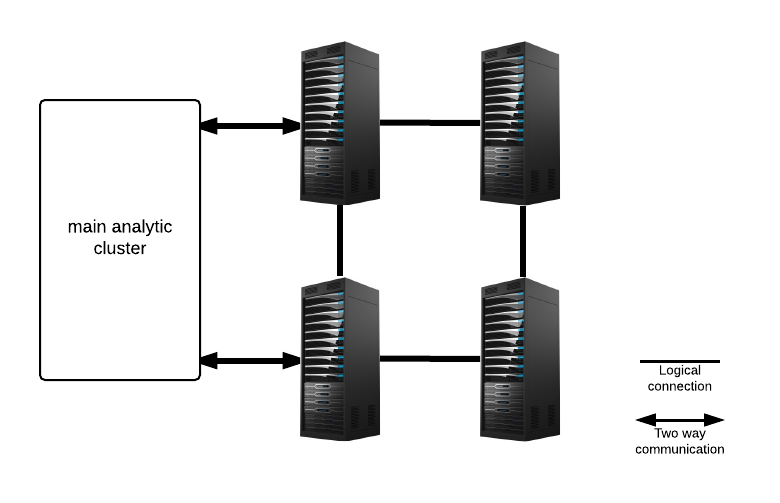
\includegraphics[width=0.7\textwidth]{6-hardware/images/db-cluster.png}
\caption{Logical schematic of database cluster of SFM}
\label{fig:database-cluster}
\end{figure}

As can be seen in \autoref{fig:database-cluster}, SFM will use four database racks to have redundancy in the system. The server is connected as a ring, which is the common way to setup database server. The database cluster By using this form of architecture, SFM will be more reliable and fault tolerant. There will also be two physical connection to the main analytic cluster to make this system more fault tolerant in terms of connection. SFM database cluster will use the same server, Dell PowerEdge R530, for controlling the SATA storage machine.

% Clustering, in the context of databases, refers to the ability of several servers or instances to connect to a single database. An instance is the collection of memory and processes that interacts with a database, which is the set of physical files that actually store data.

% Clustering offers two major advantages, especially in high-volume database environments:

% Fault tolerance: Because there is more than one server or instance for users to connect to, clustering offers an alternative, in the event of individual server failure.
% Load balancing: The clustering feature is usually set up to allow users to be automatically allocated to the server with the least load.

% Adds some picture here

\subsection{Analytics Components}
\label{subsec:analytics}
Analytics component will be the main brain of SFM. The intelligent algorithm will run on this machine. This components are also responsible for checking faulty sensors by analyzing incoming sensor data. Thus, there is a big dependency to this components. To increase availability and reliability, SFM will have six server racks to do the processing as depicted in \autoref{fig:analytic-cluster}.

\begin{figure}[H]
\centering
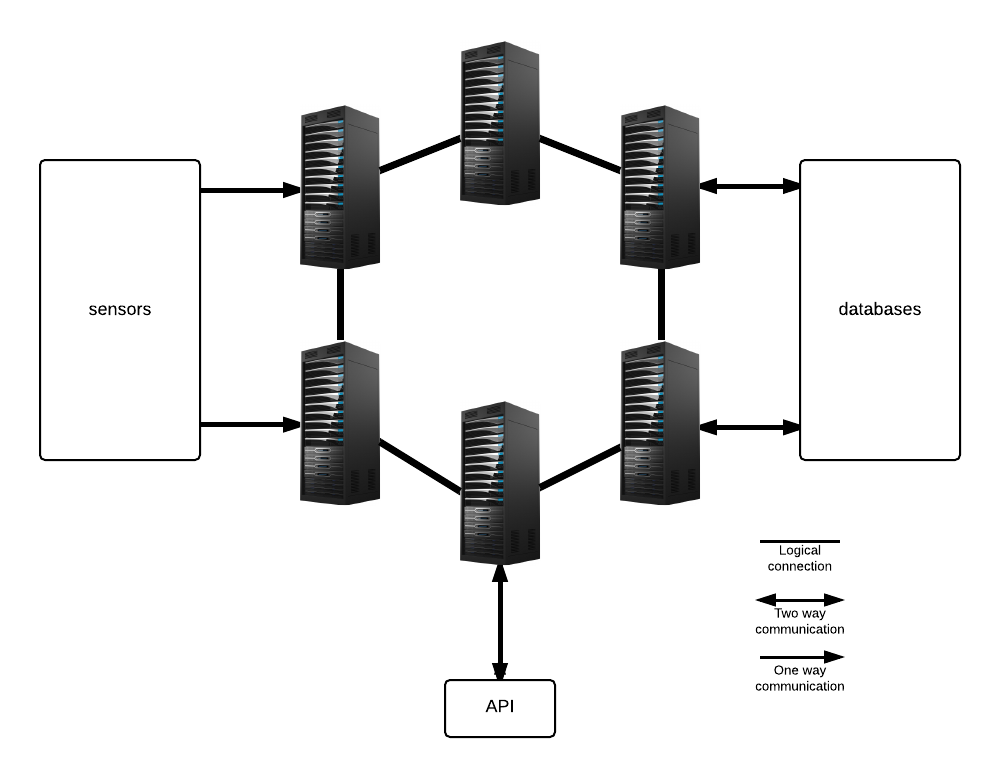
\includegraphics[width=0.7\textwidth]{6-hardware/images/analytic-cluster.png}
\caption{Logical schematic of analytic cluster of SFM}
\label{fig:analytic-cluster}
\end{figure}

The analytics components will also be the hub for the main connection of SFM. Thus, this system also need a high performance switch to accomplish this purpose. As have been mentioned before, this system will use Cisco Catalyst 2960S-24TS-L Switch.

The analytics components will use Dell PowerEdge R530 as server and it will be mounted on a server rack. The detailed hardware specifications of Dell PowerEdge R530 is listed in \autoref{table:server-specs}.
